\documentclass[12pt]{article}

\usepackage{tikz}
\usepackage{cancel}
\usepackage{amsthm}
\usepackage{amssymb}
\usepackage{amsmath}
\usepackage{latexsym}
\usepackage{mathtools}
\usepackage{stackengine}

\usepackage{fancyhdr}

\usepackage{float}
\usepackage{xcolor}
\usepackage{graphicx}
\usepackage{pagecolor}

\usepackage{soul}
\usepackage{enumerate}

\usepackage[
top=2.50cm,
bottom=2.50cm,
left=2cm,
right=2cm,
marginparsep=0pt,
marginparwidth=0pt]{geometry}

\parindent 0in
\parskip 12pt

\definecolor{Ivory Paper}{HTML}{F7F0DF}

\pagecolor{Ivory Paper}

\newcommand{\floor}[1]{\left\lfloor #1 \right\rfloor}
\newcommand{\ceil}[1]{\left\lceil #1 \right\rceil}
\newcommand{\round}[1]{\left\lfloor #1 \right\rceil}
\newcommand{\abs}[1]{\left\lvert #1 \right\rvert}
\newcommand{\sqref}[1]{[\ref{#1}]}

\newcommand{\mH}{\char"0126}
\newcommand{\mh}{\char"0127}
\newcommand{\mG}{\char"0120}
\newcommand{\mg}{\char"0121}
\newcommand{\mC}{\char"010A}
\newcommand{\mc}{\char"010B}
\newcommand{\mZ}{\char"017B}
\newcommand{\mz}{\char"017C}

\newcommand\mscriptsize[1]{\mbox{\scriptsize\ensuremath{#1}}}
\newcommand\mtiny[1]{\mbox{\tiny\ensuremath{#1}}}

\newcommand{\dfeq}{\stackrel{\text{df}}{=}}
\newcommand{\msteq}{\stackrel{\text{mst}}{=}}
\newcommand{\seqeq}{\stackrel{\text{seq}}{=}}
\newcommand{\sqemptyset}{\ensurestackMath{\stackinset{c}{}{c}{}{/}{\square}}}

\newcommand{\sqin}{%
  \mathrel{\vphantom{\sqsubset}\text{%
    \mathsurround=0pt
    \ooalign{$\sqsubset$\cr$-$\cr}%
  }}%
}

\newcommand{\seqin}{%
  \mathrel{\vphantom{<}\text{%
    \mathsurround=0pt
    \ooalign{$<$\cr$-$\cr}%
  }}%
}

\newcommand{\pp}{\mathbin{\mbox{{+}\nolinebreak\hspace{-.15em}{+}}}}

% TODO: Reorder
\DeclareMathOperator{\jtrue}{\mathbf{True}}
\DeclareMathOperator{\jdag}{dag}
\DeclareMathOperator{\jfalse}{\mathbf{False}}
\DeclareMathOperator{\jseq}{seq}
\DeclareMathOperator{\jsharedstructure}{sharedstructure}
\DeclareMathOperator{\jwalk}{walk}
\DeclareMathOperator{\jlabelwalk}{labelwalk}
\DeclareMathOperator{\jlabelwalks}{labelwalks}
\DeclareMathOperator{\jpredecessors}{predecessors}
\DeclareMathOperator{\jreachable}{reachable}
\DeclareMathOperator{\jhamiltonian}{hamiltonian}
\DeclareMathOperator{\jsimplecycle}{simplecycle}
\DeclareMathOperator{\jsimplecycles}{simplecycles}
\DeclareMathOperator{\jcycle}{cycle}
\DeclareMathOperator{\jconnected}{connected}
\DeclareMathOperator{\jweaklyconnected}{weaklyconnected}
\DeclareMathOperator{\jcycles}{cycles}
\DeclareMathOperator{\jreverse}{reverse}
\DeclareMathOperator{\jdom}{dom}
\DeclareMathOperator{\jpath}{path}
\DeclareMathOperator{\jpaths}{paths}
\DeclareMathOperator{\jdiameter}{diameter}
\DeclareMathOperator{\jrng}{rng}
\DeclareMathOperator{\jclique}{clique}
\DeclareMathOperator{\jsum}{sum}
\DeclareMathOperator{\jtree}{tree}
\DeclareMathOperator{\jitems}{items}
\DeclareMathOperator{\jwalks}{walks}
\DeclareMathOperator{\jsorted}{sorted}
\DeclareMathOperator{\jupto}{upto}
\DeclareMathOperator{\jundefined}{undefined}
\DeclareMathOperator{\jcons}{cons}
\DeclareMathOperator{\jhead}{head}
\DeclareMathOperator{\jlast}{last}
\DeclareMathOperator{\jtail}{tail}
\DeclareMathOperator{\jlen}{len}
\DeclareMathOperator{\jtotal}{total}
\DeclareMathOperator{\jfunctional}{functional}
\DeclareMathOperator{\jinjective}{injective}
\DeclareMathOperator{\jsurjective}{surjective}

\theoremstyle{plain}
\newtheorem{thm}{Theorem}
\newtheorem{cor}{Corollary}
\newtheorem{lma}{Lemma}
\newtheorem{prop}{Proposition}
\newtheorem{conj}{Conjecture}
\newtheorem{defn}{Definition}

\setlength{\headheight}{15pt}
\pagestyle{fancy}
\renewcommand{\headrulewidth}{0pt}
\lhead{J. Scerri}
\chead{Noti g\mh al \st{Qabel} Waqt l-E\.zami}
\rhead{\thepage}

% TITLE

\title{Discrete 2 (Chapter 7)\\
\vspace{0.75em}\textbf{Noti g\mh al \st{Qabel} Waqt l-E\.zami}}
\author {{\textbf{Juan Scerri}}\\
B.Sc. (Hons)(Melit.) Computing Science and Mathematics (Second Year)}

\begin{document}

\maketitle % Print the title page

\thispagestyle{empty} % Suppress headers and footers on the title page

\raggedright

\section{Relations}

\textbf{Totality:} $r \in X \leftrightarrow Y$ is said to be
total iff $\jtotal(r) \dfeq \forall\, x \in X, \exists\, y \in
Y \cdot (x, y) \in r$ it true.

\textbf{Functionality:} $r \in X \leftrightarrow Y$ is said to
be functional iff $\jfunctional(r) \dfeq\forall\, y_1, y_2 \in
Y, \forall\, x \in X \cdot (x, y_1) \in r \land (x, y_2)
\Rightarrow y_1 = y_2$ is true.

\textbf{Surjectivity:} $r \in X \leftrightarrow Y$ is said to be
surjective iff $\jsurjective(r) \dfeq\forall\, y \in Y,
\exists\, x \in X \cdot (x, y) \in r$ is true.

\textbf{Injectivity:} $r \in X \leftrightarrow Y$ is said to be
injective iff $\jinjective(r) \dfeq \forall\, x_1, x_2 \in X,
\forall\, y \in Y \cdot (x_1, y) \in r \land (x_2, y)
\Rightarrow x_1 = x_2$ is true.

\textbf{Set of Functional Relations:} $X \rightarrow Y
\dfeq \{r \in X \leftrightarrow Y : \jfunctional(r) \}$.

\section{Multisets}

\subsection{Definitions}

\textbf{Set of Multisets Over $X$:} $\mathbb{M}\,X \dfeq \{r \in
X \rightarrow \mathbb{N} : \jtotal(r)\}$.

\textbf{Empty Multiset:} $\sqemptyset \dfeq \lambda\, x \in X
\cdot 0$.

\textbf{Multiset Element Of:} $x \sqin T \dfeq T(x) > 0$

\textbf{Multiset Subset:} $T \sqsubseteq S \dfeq \forall\, x
\in X \cdot T(x) \leq S(x)$.

\textbf{Multiset Equality:} $T \msteq S \dfeq \forall\, x \in X
\cdot T(x) = S(x)$.

\textbf{Multiset Union:} $T \sqcup S \dfeq \lambda\, x \in X
\cdot T(x) + S(x)$.

\textbf{Multiset Intersection:} $T \sqcap S \dfeq \lambda\, x
\in X \cdot \min(\{T(x), S(x)\})$.

\subsection{Theorems}

\textbf{Theorem 7.4:} $T \sqcup S \msteq S \sqcup T$.

\textbf{Theorem 7.6:} $T \sqcap S \sqsubseteq T \sqcup S$.

\subsection{Exercises}

\textbf{Exercise 7.1:} $T \sqsubseteq T$ \textit{(reflexive)}
and $T \sqsubseteq R \land R \sqsubseteq S \Rightarrow T
\sqsubseteq S$ \textit{(transitive)}.

\textbf{Exercise 7.2:} $\sqemptyset \sqcap T \msteq T \sqcap
\sqemptyset \msteq \sqemptyset$ and $\sqemptyset \sqcup T \msteq
T \sqcup \sqemptyset \msteq T$.

\textbf{Exercise 7.3:} $T \sqcap T \msteq T$
\textit{(idempotent)}, $T \sqcap S \msteq S \sqcap T$
\textit{(commutative)} and $(T \sqcap S) \sqcap R \msteq T
\sqcap (S \sqcap R)$ \textit{(associative)}.

\textbf{Exercise 7.4:} $(T \sqcup S) \sqcup R \msteq T \sqcup (S
\sqcup R)$ \textit{(associative)}.

\textbf{Exercise 7.5:} $T - S \dfeq \lambda\, x \in X \cdot
\max(\{0, T(x) - S(x)\})$ \textit{(multiset difference)}, $T - T
\msteq \sqemptyset$ and $T - \sqemptyset \msteq T$.

\section{Sequences}

\subsection{Definitions}

\textbf{Finite Subsets of $\mathbb{N}$:} $\jupto(N)
\dfeq \{n \in \mathbb{N} : n < N\} = \{0, 1, \ldots, N - 1\}$.

\textbf{Set of Sequences Over $X$:} $\jseq\, X = \{s_X \in
\mathbb{N} \rightarrow X : \exists\, N \in \mathbb{N} \cdot
\jdom(s_X) = \jupto(N)\}$.

\textbf{Empty Sequence:} $\langle \rangle \dfeq \lambda\, n \in
\mathbb{N} \cdot \jundefined$.

\textbf{Head of a Sequence:} $\jhead(s_X) \dfeq s_X(0)$.

\textbf{Tail of a Sequence:} $\jtail(s_X) \dfeq \lambda\, n \in
\mathbb{N} \cdot s_X(n + 1)$.

\textbf{Cons Operator:}

$$
\jcons(x, s_X) \dfeq \lambda\, n \in \mathbb{N}
\cdot
\begin{cases}
    x          & \text{if}\ n = 0\\
    s_X(n - 1) & \text{otherwise}
\end{cases}.
$$

\textbf{Length of a Sequence:}

$$
\begin{aligned}
\jlen(s_X) &\dfeq
\begin{cases}
    0 & \text{if}\ s_X \seqeq \langle \rangle\\
    1 + \jlen(\jtail(s_X)) & \text{otherwise}
\end{cases}\\\\
&= \lambda\, n \in \mathbb{N} \cdot
\begin{cases}
    0 & \text{if}\ s_X \seqeq \langle \rangle\\
    1 + \max(\jdom(s_X)) & \text{otherwise}
\end{cases}.
\end{aligned}
$$

\textbf{Last Element of a Sequence:} $\jlast(s_X) \dfeq
s_X(\jlen(s_X) - 1)$.

\textbf{Sum of a Sequence of Natural Numbers:}

$$
\jsum(s_\mathbb{N}) \dfeq
\begin{cases}
    0 & \text{if}\ s_\mathbb{N} \seqeq \langle \rangle\\
    \jhead(s_\mathbb{N}) + \jsum(\jtail(s_\mathbb{N})) & \text{otherwise}
\end{cases}.
$$

\textbf{Sequence Concatenation:}

$$
\begin{aligned}
t_X \pp s_X &\dfeq
\begin{cases}
    s_X & \text{if}\ t_X \seqeq \langle \rangle\\
    \jcons(\jhead(t_X), \jtail(t_X) \pp s_X) & \text{otherwise}
\end{cases}\\\\
&= \lambda\, n \in \mathbb{N} \cdot
\begin{cases}
    t_X(n) & \text{if}\ n \in \jdom(t_X)\\
    s_X(n - \jlen(t_X)) & \text{otherwise}
\end{cases}.
\end{aligned}
$$

\textbf{Prefix of a Sequence:} $t_X \preceq_{p} s_X \dfeq \exists\,
r_X \in \jseq\, X \cdot t_X \pp r_X \seqeq s_X$.

\textbf{Suffix of a Sequence:} $t_X \preceq_{s} s_X \dfeq \exists\,
r_X \in \jseq\, X \cdot r_X \pp t_X \seqeq s_X$.

\textbf{Exact Subsequence:} $t_X \preceq s_X \dfeq \exists\,
r_{1_X}, r_{2_X} \in \jseq\, X \cdot r_{1_X} \pp t_X \pp r_{2_X}
\seqeq s_X$.

\subsection{Exercises}

\textbf{Exercise 7.7:} $\jlen(s_X) = 1 \Rightarrow \jhead(s_X) =
\jlast(s_X)$.

\textbf{Exercise 7.8:} $x \seqin s_X \dfeq \exists\, n \in
\mathbb{N} \cdot n \in \jdom(s_X) \land s_X(n) = x$
\textit{(sequence element of)}.

\textbf{Exercise 7.9:}

$$
\jsorted(s_X) \dfeq
\begin{cases}
    \jtrue & \text{if}\ \jlen(s_X) \leq  1\\
    \jhead(s_X) \leq_{X} \jhead(\jtail(s_X)) \land
    \jsorted(\jtail(s_X)) & \text{otherwise}
\end{cases}.
$$

\textbf{Exercise 7.10:} $\jitems \dfeq \lambda\, s_X \in \jseq\,
X \cdot (\lambda\, x \in X \cdot \#\{n \in \mathbb{N} : s_X(n) =
x\})$.

\textbf{Exercise 7.11:} $\operatorname{sorts} \dfeq \{(s_X,
s_X') \in \jseq\, X \times \jseq\, X : \jitems(s_X) \msteq
\jitems(s_X') \land \jsorted(s_X) \}$. Hence, $(s_X, s_X') \in
\operatorname{sorts}$ iff $s_X$ is a sorted version of $s_X'$.

\textbf{Exercise 7.12:} $s_X \seqeq s_X' \dfeq \jlen(s_X) =
\jlen(s_X') \land \forall\, n \in \mathbb{N} \cdot n \in
\jupto(\jlen(s_X)) \Rightarrow s_X(n) = s_X'(n)$. 

\textbf{Exercise 7.13:}

\begin{enumerate}[(i)]
    \item $\jreverse(s_X) \dfeq
        \begin{cases} s_X & \text{if}\
            \jlen(s_X) \leq 1\\ \jreverse(\jtail(s_X)) \pp
            \jcons(\jhead(s_X), \langle \rangle) & \text{otherwise}
        \end{cases}.$
    \item $\jreverse(s_X) \dfeq \lambda\, n \in \mathbb{N} \cdot
        s_X(\jlen(s_X) - (n + 1))$.
\end{enumerate}

\section{Graph Theory}

\subsection{Definitions}

\textbf{Directed Multigraph:} $G$ is said to be a directed
multigraph iff $G = (V, L, E)$ where $E \subseteq V \times L
\times V$.

\textbf{A Clique in $G$:} $V' \subseteq V$ is said to be a clique iff
$\jclique(V') \dfeq \forall\, v, v' \in V' \cdot v \neq v'
\Rightarrow (\exists\, l \in L \cdot (v, l, v') \in E)$ is true.

\textbf{A Walk in $G$:} $s_V \in V$ is said to be a walk iff
$\jwalk(s_V) \dfeq \forall\, n \in \mathbb{N} \cdot n \in
\jupto(\jlen(s_V) - 1) \Rightarrow (\exists\, l \in L \cdot
(s_V(n), l, s_V(n + 1) \in E)$ is true.

\textbf{Set of Walks in $G$:} $\jwalks(G) \dfeq \{s_V \in
\jseq\, V : \jwalk(s_V)\}$.

\textbf{A Cycle in $G$:} $s_V \in V$ is said to be a cycle iff
$\jcycle(s_V) \dfeq \jwalk(s_V) \land \jhead(s_V) = \jlast(s_V)$
is true. 

\textbf{Set of Cycles in $G$:} $\jcycles(G) \dfeq \{s_V \in
\jseq\, V : \jcycle(s_V)\}$.

\textbf{Directed Acyclic Graph (DAG):} $G$ is said to be a DAG
iff $\jdag(G) \dfeq \jcycles(G) = \emptyset$ is true. 

\textbf{Set of Predecessors of $v$:} $\jpredecessors(v) \dfeq \{v'
\in V : \exists\, l \in L \cdot (v', l, v) \in E\}$.

\textbf{Set of Vertices Reachable from $v$:} $\jreachable(v) \dfeq \{v'
\in V : \exists s_V \in \jseq\, V \cdot \jwalk(s_V)
\land \jhead(s_V) = v \land \jlast(s_V) = v'\}$.

\textbf{Tree:} $G$ is said to be a tree iff $\jtree(G) \dfeq
(\forall\, v \in V \cdot \#\jpredecessors(v) \leq 1) \land
(\exists_{1}\, v \in V \cdot \#\jpredecessors(v) = 0) \land
(\forall\, v \in V \cdot \#\jpredecessors(v) = 0 \Rightarrow
\jreachable(v) = V)$ is true.

\textbf{A Label Walk in $G$:} $s_L \in \jseq\, L$ is said to be
a label walk iff $\exists\, s_V \in \jseq\, V \cdot
\jlabelwalk(s_L, s_V) \dfeq \jwalk(s_V) \land \jlen(s_V) =
\jlen(s_L) + 1 \land (\forall\, n \in \mathbb{N} \cdot n \in
\jupto(\jlen(s_V) - 1) \Rightarrow (s_V(n), s_L(n), s_V(n + 1))
\in E)$ is true.

\textbf{Set of Label Walks in $G$:} $\jlabelwalks(G) \dfeq
\{(s_L, s_V) \in \jseq\, L \times \jseq\, V : \jlabelwalk(s_L,
s_V)\}$.

\textbf{Travelling Salesman Problem (TSP):} Let $G = (V,
\mathbb{N}, E)$ and suppose a buget $B$, is the following
predicate true? $\exists\, (s_L, s_V) \in \jlabelwalks(G) \cdot
\operatorname{ran}(s_V) = V \land \jsum(s_L) \leq B$.

\textbf{Boolean Satisfiability Problem (SAT):} Consider the
following boolean expression:

$$
\begin{aligned}
&\ (P \vee Q \vee R)\\
\land &\ (\neg P \vee \neg R)\\
\land &\ (P \vee R \vee \neg Q)
\end{aligned}
$$

$$\big\downarrow$$

\begin{center}
    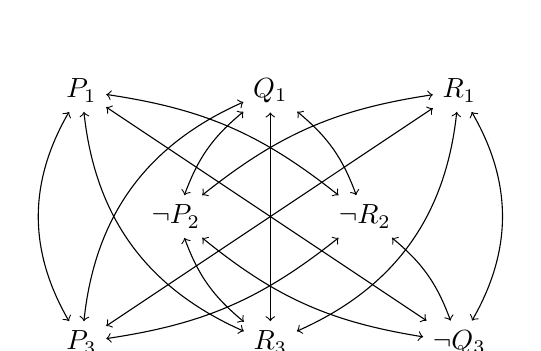
\begin{tikzpicture}
        [scale=.8,auto=center]

        \node (p1) at (0,4) {$P_1$};
        \node (q1) at (3,4) {$Q_1$};
        \node (r1) at (6,4) {$R_1$};
        \node (p2) at (1.5,2) {$\neg P_2$};
        \node (r2) at (4.5,2) {$\neg R_2$};
        \node (p3) at (0,0) {$P_3$};
        \node (r3) at (3,0) {$R_3$};
        \node (q3) at (6,0) {$\neg Q_3$};
        
        \draw[to-to] (p1) edge (q3);
        \draw[to-to] (p1) edge [bend left = 1.5em] (r2);
        \draw[to-to] (p1) edge [bend right = 3em] (r3);
        \draw[to-to] (p1) edge [bend right = 3em] (p3);

        \draw[to-to] (q1) edge [bend left = 1.5em] (r2);
        \draw[to-to] (q1) edge [bend right = 1.5em](p2);
        \draw[to-to] (q1) edge (r3);
        \draw[to-to] (q1) edge [bend right = 3em] (p3);

        \draw[to-to] (r1) edge (p3);
        \draw[to-to] (r1) edge [bend right = 1.5em] (p2);
        \draw[to-to] (r1) edge [bend left = 3em] (r3);
        \draw[to-to] (r1) edge [bend left = 3em] (q3);

        \draw[to-to] (p2) edge [bend right = 1.5em] (r3);
        \draw[to-to] (p2) edge [bend right = 1.5em] (q3);

        \draw[to-to] (r2) edge [bend left = 1.5em] (q3);
        \draw[to-to] (r2) edge [bend left = 1.5em] (p3);
    \end{tikzpicture}
\end{center}

Vertices on the same level e.g. $P_1$ and $Q_1$ are not
connected. Additionally, complementary vertices e.g. $P_1$ and
$\neg P_2$ are not connected.

Finding a clique corresponds to a solution for the boolean
expression e.g. $Q_1$, $\neg P_2$ and $R_3$. This means SAT is
as hard as finding cliques.

\subsection{Exercises}

\textbf{Exercise 7.14:} $\jhamiltonian(s_V) \dfeq \forall\, v
\in V, \exists_{1}\, n \in \mathbb{N} \cdot s_V(n) = v$.

\textbf{Exercise 7.15:} $\jsimplecycle(s_V) \dfeq \jcycle(s_V)
\land \#\jrng(s_V) + 1 = \jlen(s_V)$, $\jsimplecycles(G) \dfeq
\{s_V \in \jseq\, V : \jsimplecycle(s_V)\}$.

\textbf{Exercise 7.16:} $\jpath(s_V) \dfeq \jwalk(s_V) \land
\#\jrng(s_V) = \jlen(s_V)$, $\jdiameter(G) \dfeq \max(\{s_V \in
\jseq\, V : \jpath(s_V) \cdot \jlen(s_V)\})$.

\textbf{Exercise 7.17:}

\begin{enumerate}[(i)]
    \item $\hat{E} \dfeq \{(v, l, v') \in V\times L \times V :
        (v, l, v') \in E \cdot (v', l, v)\}$, $\hat{G} \dfeq (V,
        L, E \cup \hat{E})$ \textit{(undirected $G$)}.
    \item $\jconnected(G) \dfeq \forall\, v, v' \in V, \exists\,
        s_V \in \jseq\, V \cdot \jpath(s_V) \land \jhead(s_V) =
        v \land \jlast(s_V) = v'$, $\jweaklyconnected(G) \dfeq
        \jconnected(\hat{G})$.
    \item $\jsharedstructure(G) \dfeq \exists\, v, v' \in V,
        \exists\, s_V, s_V' \in \jseq\, V \cdot \jpath(s_V)
        \land \jpath(s_V') \land \neg(s_V \seqeq s_V') \land
        ((\jhead(s_V) = \jhead(s_V') = v \land \jlast(s_V) =
        \jlast(s_V') = v') \vee (\jhead(s_V) = \jlast(s_V') = v
        \land \jlast(s_V) = \jhead(s_V') = v'))$ \textit{(at
        least two vertices are joined by two distinct paths)}.
    \item $\jtree(G) \dfeq \jdag(G) \land \jweaklyconnected(G)
        \land \neg \jsharedstructure(G)$.
\end{enumerate}

\end{document}
